\documentclass{article}

\usepackage[utf8x]{inputenc}
\usepackage[T1]{fontenc}
\usepackage[francais]{babel}
\usepackage{xcolor}
\usepackage{listings}
\usepackage{mathptmx}
\usepackage{anyfontsize}
\usepackage{t1enc}
\usepackage[top=2cm, bottom=2cm, left=2cm, right=2cm]{geometry}
\usepackage{titlesec}
\usepackage{titling}
\usepackage{graphicx}
\usepackage{pgfplots}
\usepackage{csquotes}
\usepackage[colorlinks = true,
            linkcolor = black,
            urlcolor  = black,
            citecolor = black,
            anchorcolor = black]{hyperref}

\newcommand{\changeurlcolor}[1]{\hypersetup{urlcolor=#1}}

\renewcommand\maketitlehooka{\null\mbox{}\vfill}
\renewcommand\maketitlehookd{\vfill\null}

\definecolor{codegreen}{rgb}{0,0.6,0}
\definecolor{codegray}{rgb}{0.5,0.5,0.5}
\definecolor{codepurple}{rgb}{0.58,0,0.82}
\definecolor{backcolour}{rgb}{0.95,0.95,0.92}
\definecolor{codekeywords}{rgb}{0.1,0.53,0.92}

\lstdefinestyle{c++}{
    backgroundcolor=\color{backcolour},   
    commentstyle=\color{codegreen},
    keywordstyle=\color{codekeywords},
    numberstyle=\tiny\color{codegray},
    stringstyle=\color{codepurple},
    basicstyle=\ttfamily\footnotesize,
    breakatwhitespace=false,         
    breaklines=true,                 
    captionpos=b,                    
    keepspaces=true,                 
    numbers=left,                    
    numbersep=5pt,                  
    showspaces=false,                
    showstringspaces=false,
    showtabs=false,                  
    tabsize=2,
    texcl=false,
    inputencoding=utf8,
    extendedchars=true,
    literate=
  {á}{{\'a}}1 {é}{{\'e}}1 {í}{{\'i}}1 {ó}{{\'o}}1 {ú}{{\'u}}1
  {Á}{{\'A}}1 {É}{{\'E}}1 {Í}{{\'I}}1 {Ó}{{\'O}}1 {Ú}{{\'U}}1
  {à}{{\`a}}1 {è}{{\`e}}1 {ì}{{\`i}}1 {ò}{{\`o}}1 {ù}{{\`u}}1
  {À}{{\`A}}1 {È}{{\'E}}1 {Ì}{{\`I}}1 {Ò}{{\`O}}1 {Ù}{{\`U}}1
  {ä}{{\"a}}1 {ë}{{\"e}}1 {ï}{{\"i}}1 {ö}{{\"o}}1 {ü}{{\"u}}1
  {Ä}{{\"A}}1 {Ë}{{\"E}}1 {Ï}{{\"I}}1 {Ö}{{\"O}}1 {Ü}{{\"U}}1
  {â}{{\^a}}1 {ê}{{\^e}}1 {î}{{\^i}}1 {ô}{{\^o}}1 {û}{{\^u}}1
  {Â}{{\^A}}1 {Ê}{{\^E}}1 {Î}{{\^I}}1 {Ô}{{\^O}}1 {Û}{{\^U}}1
  {œ}{{\oe}}1 {Œ}{{\OE}}1 {æ}{{\ae}}1 {Æ}{{\AE}}1 {ß}{{\ss}}1
  {ç}{{\c c}}1 {Ç}{{\c C}}1 {ø}{{\o}}1 {å}{{\r a}}1 {Å}{{\r A}}1
  {€}{{\EUR}}1 {£}{{\pounds}}1,
}
\lstset{style=c++}


\title{Simulation TP5\\Cahier des charges Système Multi-Agents}
\author{Arquillière Mathieu - Zangla Jérémy}
\date{\today}

\begin{document}

\begin{titlepage}
  \maketitle
\end{titlepage}

\tableofcontents
\listoffigures
\newpage

\section{Introduction}
L'objectif ici est de réaliser un système multi-agents simple, afin d'en
comprendre et d'expérimenter les difficultés et les intérêts.

Notre problèmatique est donc :

\enquote{Quels agents créer et comment les intégrer dans un système afin
qu'ils interagissent entre eux et avec l'environnement}.
Cette problèmatique implique de comprendre comment un ensemble d'agents doit agir
en simultané dans un même espace (en 2 dimensions dans notre cas).

\section{Interface}
Le système multi-agents pourra être utilisé de manière très simple. C'est-à-dire
que l'interface consistera à pouvoir lancer une simulation en réglant des paramètres
comme l'endroit d'apparition des agents / bases / ressources et de leurs nombres. On
pourra également modifier la vie des agents \emph{mangeurs} et les probabilitées des
types de ressources.

Une autre partie importante est de pouvoir récuperer des informations, des statistiques
sur les systèmes qu'on observe. Ainsi notre système enregistrera certaines données
au fur et à mesure de son évolution et pourra les exporter (sous forme de fichier
par exemple).

\begin{figure}[!ht]
  \centering
  \caption{Diagramme cas d'utilisation}
  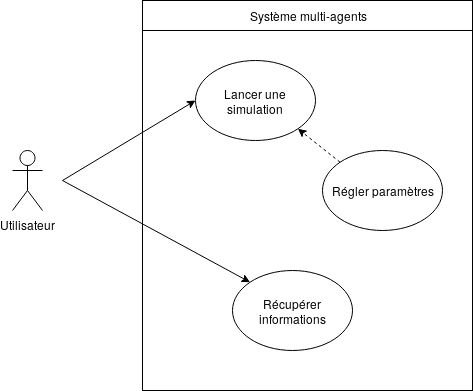
\includegraphics[scale=0.70]{img/usecase.png}
\end{figure}

\section{Modélisation}
\subsection{Agents}
Notre système se composera de 2 types d'agents:
\begin{itemize}
  \item les \emph{récolteurs}
  \item les \emph{mangeurs}
\end{itemize}

\subsubsection{Récolteurs}
L'objectif de cet agent est récolter des ressources et de les ramener à sa base. Chaque
agent de ce type a été créé par une \emph{case particulière} de l'environnment qu'on
appelera sa \emph{base}. Un \emph{récolteur} bouge aléatoirement dans l'espace
en 2 dimensions. Lorqu'il trouve une case avec des ressources, il la prend et se déplace
alors vers leur base (ce qui implique que ces agents savent à tous moments l'endroit de
leur base). Une fois dessus, il dépose ses ressources et se remet en recherche.

Les \emph{récolteurs} naissent grâce à une base. Lorsqu'une base possède assez de ressources,
elle les consomme et créé un nouvel agent \emph{récolteur}.

\begin{figure}[!ht]
  \centering
  \caption{Diagramme état-transition de l'agent \emph{récolteur}}
  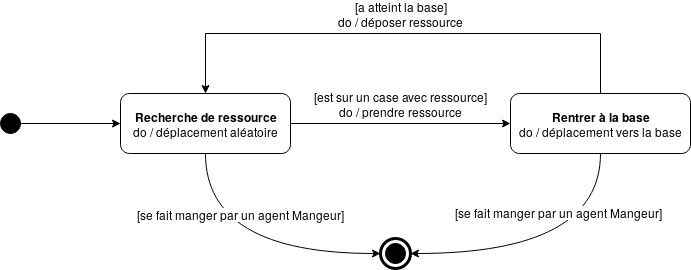
\includegraphics[scale=0.70]{img/etat-transition_recolteur.png}
\end{figure}

\subsubsection{Mangeurs}
L'objectif de cet agent est de manger des agents \emph{récolteurs} afin de survivre.
Il se déplace aléatoirement jusqu'à ce qu'il trouve dans un voisinage de Moore d'ordre 3
un agent \emph{récolteur}. Dès lors, il se déplace vers celui-ci (ses déplacements se
font dans un voisinage de Moore d'ordre 2). Si il atteint un \emph{récolteur} (être
sur la même case de l'esapce 2D) alors il le détruit.

Le \emph{mangeur} possède une "barre de vie" qui diminue à chaque nouvel état du système.
Manger un \emph{récolteur} permet de regagner de la vie. Si il en mange un alors que sa
vie était assez haute (exemple: > 90\%) alors il créé un nouvel agent \emph{mangeur}.

\begin{figure}[!ht]
  \centering
  \caption{Diagramme état-transition de l'agent \emph{mangeur}}
  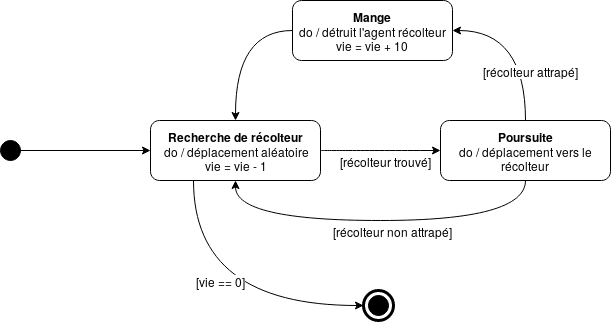
\includegraphics[scale=0.70]{img/etat-transition_mangeur.png}
\end{figure}

\subsection{Environnement}
L'environnement sera une matrice (20x20 à la base). Une case de cette matrice peut:
\begin{itemize}
  \item être vide
  \item contenir un agent
  \item contenir une ressource
  \item contenir une base
\end{itemize}

\subsubsection{Elements de l'environnement utiles au agents}

Une ressource a une position dans l'espace 2D et a un type : faible, moyen ou fort et
correspond à une quantité pour les bases. Tous les certains temps du système, un certain
nombre de ressources apparaissent aléatoirement dans l'espace.

Une base intéragit avec des agents \emph{récolteurs}. Elle possède une position fixe
dans l'espace 2D et s'occupe de créer des \emph{récolteurs}. En effet ceux-ci rapporte
à la base des ressources qui, au dessus d'un certain seuil, sont consommées afin de
générer un nouvel agent \emph{récolteur}.

\newpage
\subsection{Diagramme de classe}
Afin de mieux comprendre les relations entre les agents et leur environnement, on
réalise un diagramme de classe non détaillé, qui sera ensuite complété et modifié
lors de l'implémentation.

\begin{figure}[!ht]
  \centering
  \caption{Diagramme de classe du système multi-agents}
  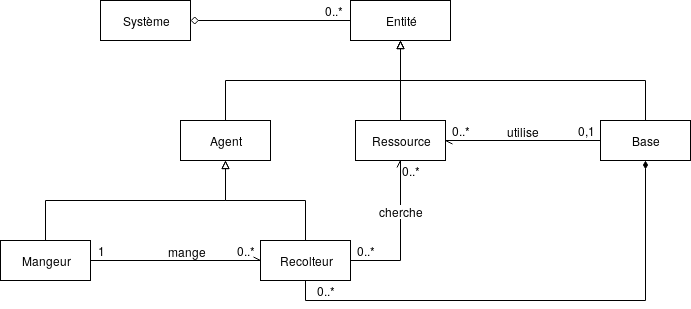
\includegraphics[scale=0.70]{img/class_agents.png}
\end{figure}

\end{document}